%% Figure from MATH 556 notes, section 48 (Lecture 21). board sketch (Lecture 21), redrawn.
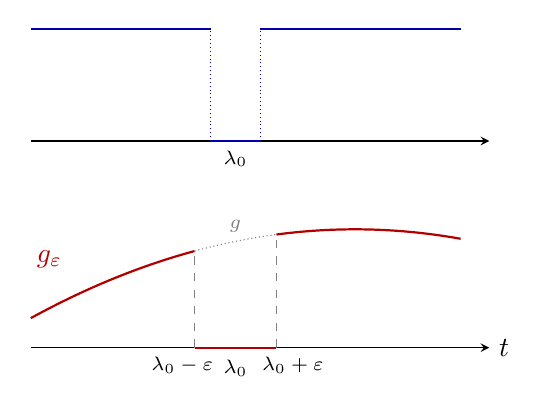
\begin{tikzpicture}[>=stealth, xscale=5.2, yscale=1.5]
    \begin{scope}[shift={(0,1.75)}]
        \draw[->] (0,0) -- (1.12,0);
        \draw[thick, blue!65!black] (0,0.95) -- (0.44,0.95);
        \draw[thick, blue!65!black] (0.56,0.95) -- (1.05,0.95);
        \draw[thick, blue!65!black] (0.44,0) -- (0.56,0);
        \draw[densely dotted, blue!65!black] (0.44,0) -- (0.44,0.95);
        \draw[densely dotted, blue!65!black] (0.56,0) -- (0.56,0.95);
        \node[below, font=\scriptsize] at (0.5,0) {$\lambda_0$};
    \end{scope}
    \draw[->] (0,0) -- (1.12,0) node[right] {$t$};
    \draw[thick, red!70!black, domain=0:0.4, samples=40, smooth] plot (\x, {0.25+1.9*\x-1.2*\x*\x});
    \draw[thick, red!70!black, domain=0.6:1.05, samples=40, smooth] plot (\x, {0.25+1.9*\x-1.2*\x*\x});
    \draw[thick, red!70!black] (0.4,0) -- (0.6,0);
    \draw[gray, densely dotted, domain=0.4:0.6, samples=20] plot (\x, {0.25+1.9*\x-1.2*\x*\x});
    \draw[dashed, gray] (0.4,0) -- (0.4,0.818);
    \draw[dashed, gray] (0.6,0) -- (0.6,0.958);
    \node[below, font=\scriptsize] at (0.37,0) {$\lambda_0 - \varepsilon$};
    \node[below, font=\scriptsize] at (0.5,-0.02) {$\lambda_0$};
    \node[below, font=\scriptsize] at (0.64,0) {$\lambda_0 + \varepsilon$};
    \node[red!70!black, anchor=east] at (0.1,0.75) {$g_\varepsilon$};
    \node[gray, font=\scriptsize] at (0.5,1.03) {$g$};
\end{tikzpicture}
